\documentclass[12pt]{article}
\linespread{1.3}
\usepackage{amsmath}
\usepackage[margin=1in]{geometry}
\usepackage{graphicx}
\usepackage{dirtytalk}
\title{Master Project - Comparing the Spatial Scanning Methods and a Connection to Graph Theory  }
\author{Duong Than}
\date{\today}
\begin{document}
\maketitle	
	
		\section{Introduction :} 
		\subsection{Background} 

			Public health officials are interested in finding hotspots where disease risks is unusually high. They want to immediately identify any disease clusters and also potential disease hotspots in order to implement prevention programs before the outbreak turns into an epidemic. \\ 		
			
			Consequently, researchers have developed different methods to detect disease clusters, and there are many ideas that used developed point and regional count data to come up with an optimized solution. \\
			
			\textbf{What is a hotspot or a cluster?} A disease cluster defined as a collection of connected regions that has an unusually high proportion of observed cases to expected cases.Practically, there are more cases in those regions than we would expect if disease risk is constant over all regions.\\
			
			\textbf{An example of an appearance of disease clusters:} There is a state where certain counties  have an abnormally high number of observed cases. Public health officials worry about the uncontrolled spread of this disease, so they want to know exactly where the observed cases are significantly high and where there could be the hotspots. A comparison between the observed cases and the population of each region is made. So our ideal solution is to find some zones (could be more than one connected regions) where the observed cases are significantly large, and the rest of the zones are not significantly high. Ideally, we would consider all connected zones as a hotspot. However, if the number of regions is large, it is not feasible for us to be able to find all the connected regions within the study area. Instead we need to come up with clever ways to find some \say{reasonable} subsets of regions to consider as potential hotspots. Furthermore, with respect to statistics, there are some restrictions for our zones. Since we do not want to consider a zone with many regions and with a very large population,each zone has a limit for the number of regions and the total population of each zone has to be less than or equal a half of the entire study area's population. These restrictions help us to reduce the size of possible zones of the entire study area. However; datasets can be varying in many ways, we still need to come up with more clever methods of finding appropriate zones to detect for clusters. \\       
			
			\textbf{Objectives:} One of the main purposes of this paper is to compare and contrast three existing methods for detecting hotspots. Also we want to approach this problem from a graph theory point of view. In addition to this, we will propose some improvements for these methods. But first, we want to introduce the type of dataset we will consider. \\
				
		\subsection{Data Structure:} 
			In this section, we go into more detail about the data typically observed and standard assumptions about the dataset. 
			The basic form of the data involves a set of \textit{counts observed} (one count for each region ) and a matching set of \textit{counts expected} reporting the number of cases we expect in each region, under the null hypothesis that everyone in the entire study area has the same constant risk. \\
			
We often assume that the data represent a set of counts arising from a \textbf{Heterogeneous Poisson process}.
In particular, many methods model the regional counts as independent Poisson random variables based on one of the basic properties of a spatial Poisson process: event counts from non overlapping regions follow independent Poisson distributions based on an underlying intensity function defining the expected values (and variances). Also, the counts are non negative and discrete, which are the two main properties of Poisson distribution. \\
			 
			
			
			As an example of the structure of a spatial dataset of regional counts, we consider a Leukemia dataset for 218 regions in New York. This dataset contains 218 observations related to leukemia cases in 8 counties in the state of New York. The data were made available in Waller and Gotway (2005) and details are provided there. In this paper, we study geographical regions and their connected neighbors.		
The graphics below is illustrating a study area and the regions in it. For example, suppose we want to look at center region 83, and we want to study its five nearest neighbors. The algorithm to determine the nearest neighbors is to use the Euclidean distance to find the five centroids that have closest distances to centroid 83. Thus the five nearest regions of region 83 which are 89,90,84,88, and 75. We successively consider region 83 and its five nearest neighbors in figure: \\	
	\newpage
	
		\begin{figure}[!ht]	
		\begin{tabular}{|c|c|c|}
			\hline
			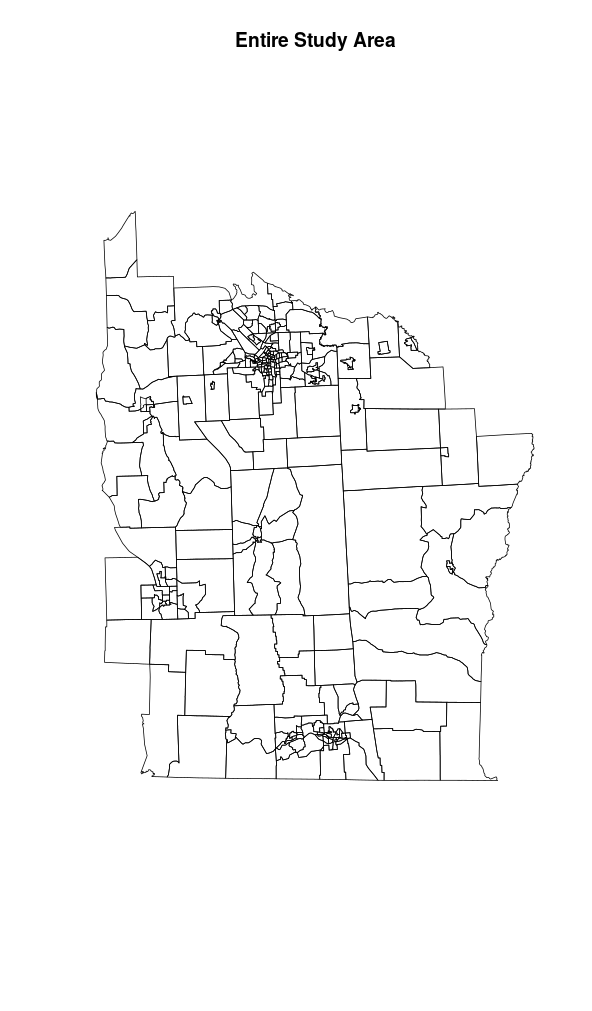
\includegraphics[scale=0.18]{nyplot.png}
			  & 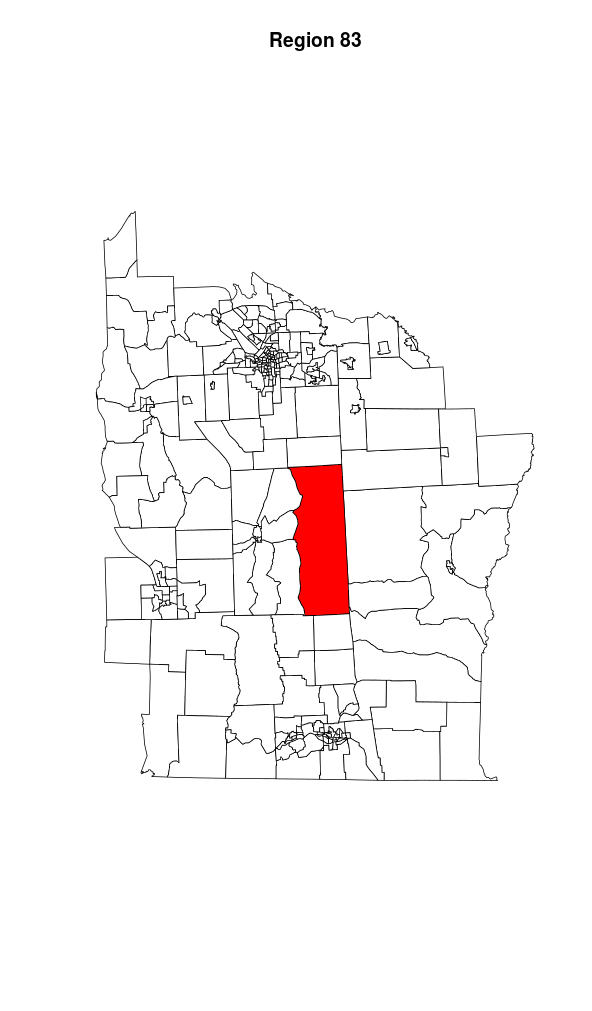
\includegraphics[scale=0.18]{ny83.png}
					&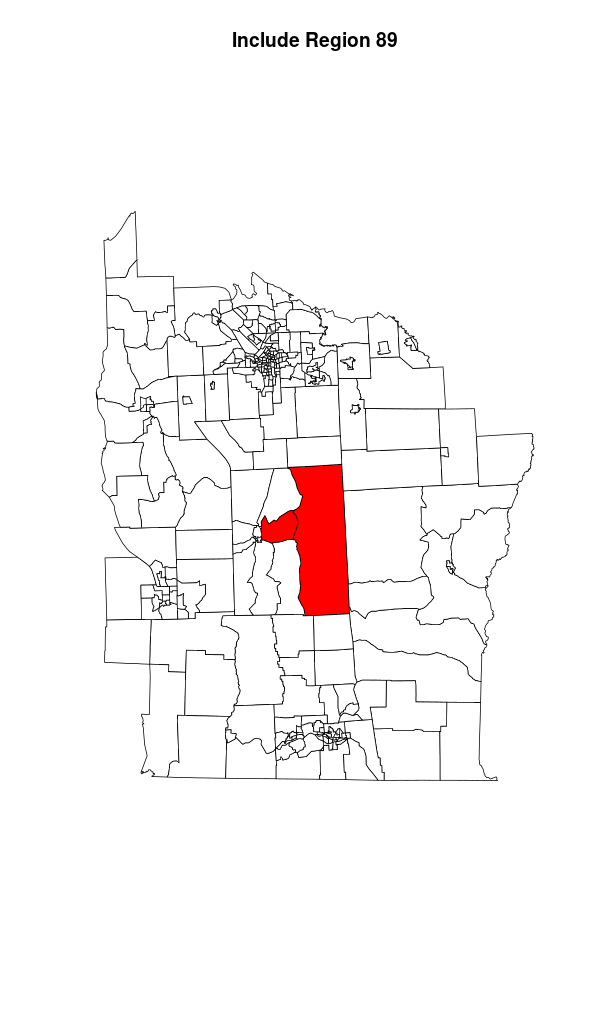
\includegraphics[scale=0.18]{ny89.png} \\ \hline
						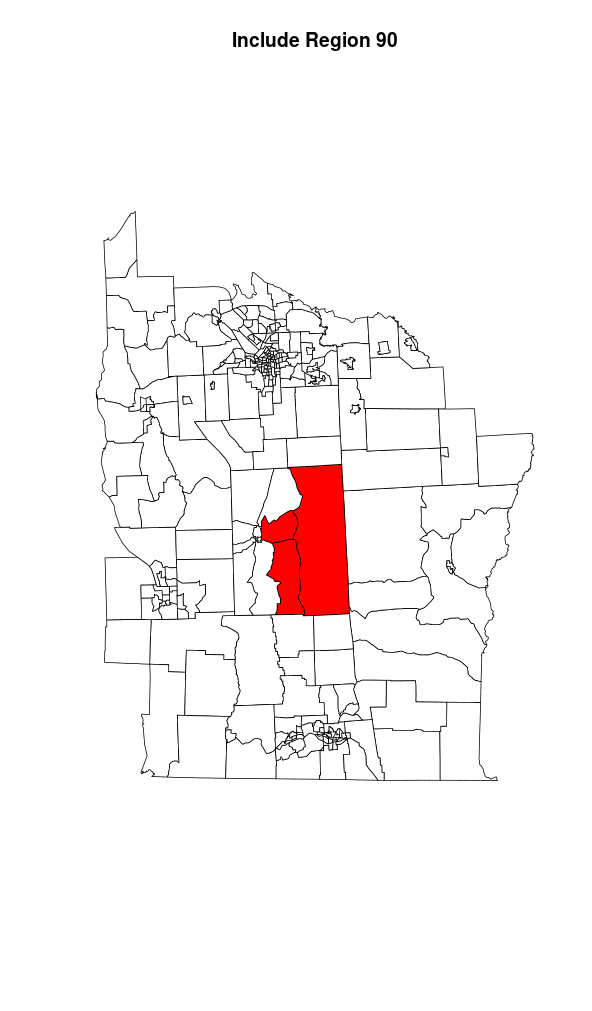
\includegraphics[scale=0.18]{ny90.png}
							& 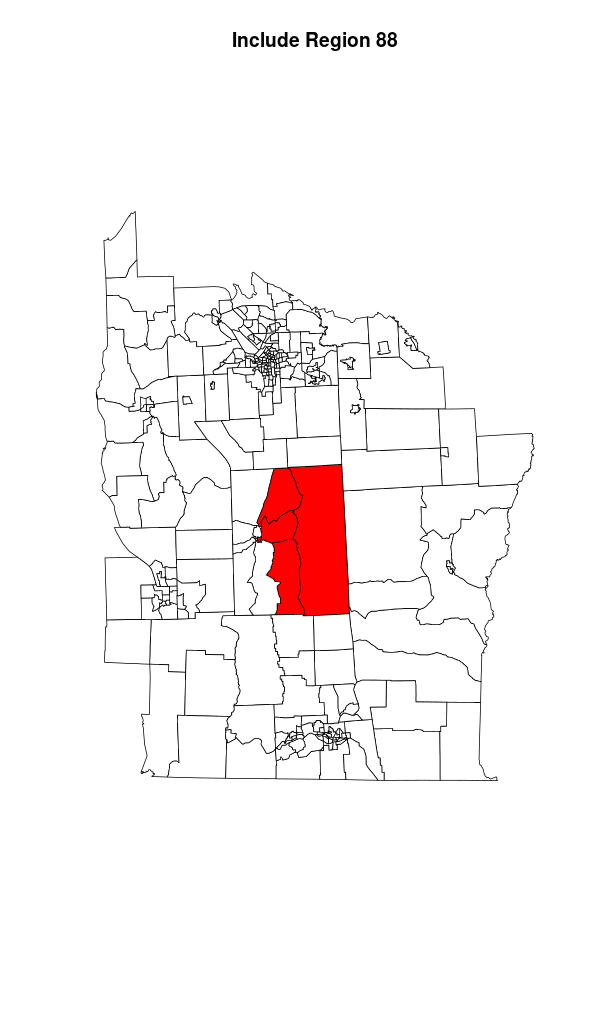
\includegraphics[scale=0.18]{ny88.png}
							   & 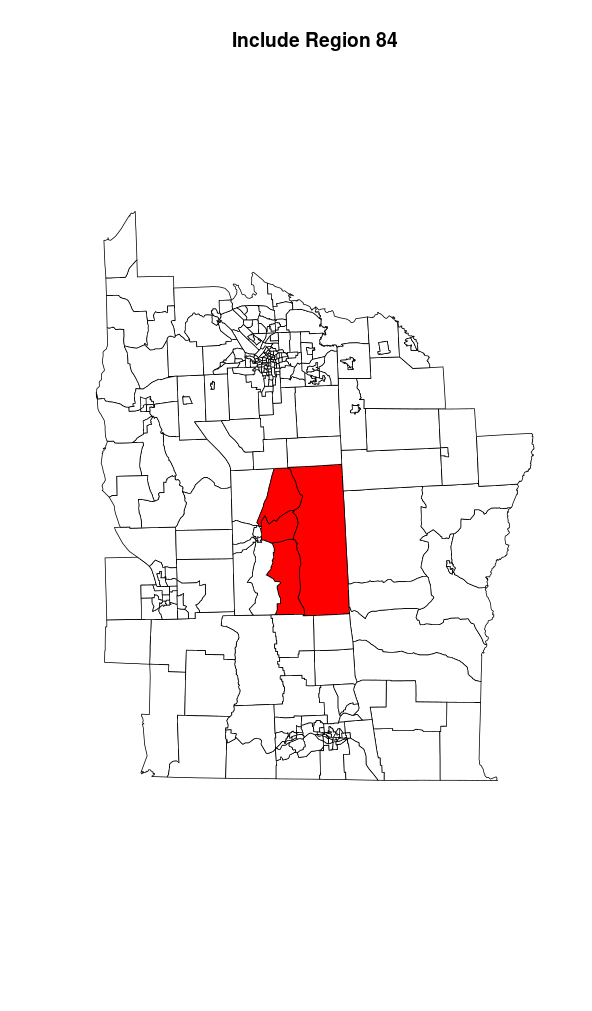
\includegraphics[scale=0.18]{ny84.png} \\ \hline
									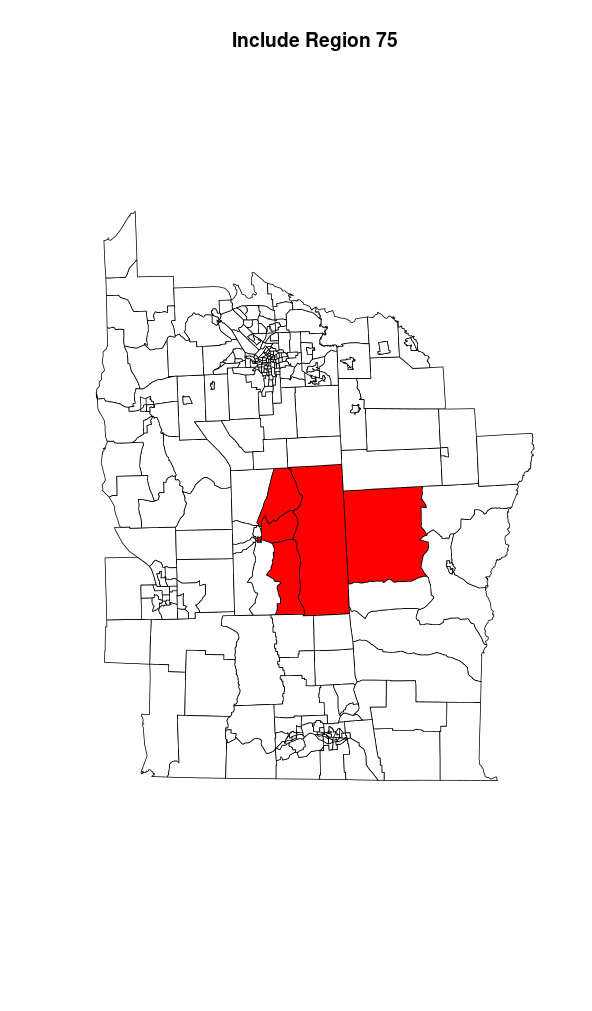
\includegraphics[scale=0.18]{ny75.png} && \\
		\hline	
		
		\end{tabular}	\\
		\caption{Region 83 and its five nearest regions. \label{f:gull}}
		\end{figure}	
			\newpage
			The data $Y_1,Y_2,\dots,Y_N$ in regions $1,2,\dots,N$ are mutually independent Poisson random variables, where $Y_i$ are the observed cases in region $i$. \\ 
			The associated population of each region is $n_1,n_2,\dots,n_N$. In this problem, we want to use the counts observed in each region to determined where the risk is unusually high.\\
Table below is an example of a dataset, which include region 83 and its five nearest neighbors, was extracted from the Leukemia New York dataset: \\

		\begin{tabular}{|c|c|c|c|}
		\hline
		Region & Population $(n_i$)& Observed Cases $(Y_i)$ & \\ 
		83 & 5532& 3.33995 & \\
		89 & 2921& 8.1795 & \\
		90 & 3711& 5.22804 & \\
		84 & 2592& 1.15928 & \\
		88 & 3242& 2.19922 & \\
		75 & 4189& 0.50936 & \\
		\hline
		\end{tabular}\\
			
			\subsection{Method:} 

			For the most part, methods to assess clusters and clustering in count data assume some background information on the entire population rather than a set of controls. 
			We divide the entire study area into N regions $ i = \{1,2,\dots,N\}$. \\
			Since we consider the population sizes $n_1,n_2,\dots,n_N$ fixed ,the total population in the study area, \\
\[
n_+ = \sum_{i =1}^{N}n_i,
\]
is also fixed. \\
Let $Y_+ = \sum_{i=1}^{N} Y_i$. If we condition on $n_+$, the total number of observed cases, we get the probability $ r = \dfrac{Y_+}{n_+}$, which is a fixed constant risk for all the individuals under the constant risk hypothesis (CRH).\\
		
			\textbf{Test Hypothesis :} \\ 
			Let $Z$ be a collection of connected regions which we call a zone. \\
			We define $Y_+(Z) = \sum_{i \in Z} Y_i$ , $n_+(Z)=\sum_{i \in Z} n_i$ and $E(Z) = r*n_+(Z)$. \\
			
			\textit{Null hypothesis :} The number of observed cases for each region equals the expected number of cases. \\ 
			\begin{center}
			$H_0 : r_i = r$ for all $i$
			 \end{center}
			
			
			
			\textit{Alternative hypothesis :} There is at least one zone for which the underlying risk is higher when compared to the null hypothesis. \\
 			\begin{center}
			$H_1$ : $r_i \geq r$. \\
			\end{center}	
			With the assumption of Poission Process, below is the test statistic of likelihood ratio test for spatial clustering developed by Kulldorff : \\
				\[
					T = \max_{z\in Z} \bigg[\dfrac{Y_+(Z)}{E(Z)}\bigg]^{Y_+(Z)} \bigg[\dfrac{Y_+(Z^c)}{E(Z^c)}\bigg]^{Y_+(Z^c)} I\bigg[\dfrac{Y_+(Z)}{E(Z)} > \dfrac{Y_+(Z^c)}{E(Z^c)}\bigg]
				\]	  (1)
		
				where $ Z^c$ denotes all the regions outside zone Z, Y() denotes the observed cases within a zone, and $I()$ is the indicator function. \\ 
			
			 \textit{Commentary}: A zone is considered as cluster when its T-value is high enough so that it has to be statistically significant at the 0.05 level. Note that different techniques of picking potential clusters resulted in different T-values and T-value thresholds which determine whether clusters are statistically significant. \\
			 
			 \textbf{To determine significance:} \\
			 \begin{enumerate}
			 	
			 \item First, we generate a certain number (i.e. 99,999,9999,etc ) of simulated datasets under the constant risk hypothesis(CRH).
			 
			 \item We calculate the largest test statistic across all candidate zones for each of the sample. This step helps us to form the null distribution of the test statistic.
			 
			 \item Next, we calculate the test statistics for the observed data. The statistics are sorted from largest to smallest.  Candidate zones that intersect another candidate zone with a larger test statistic are removed from consideration.\\
			 
			 \end{enumerate}
			
			P-values are calculated for each remaining candidate zone.  The p-value is the probability of observing a more extreme maximal statistic anywhere in the study area.  The p-value for each candidate zone is computed as the proportion of simulated data sets for which the maximum test statistic was at least as large as the observed test statistics.\\
			
			\textbf{Restrictions for a target zone : } As we mentioned earlier, philosophically there are some restrictions for clusters. For each region's centroid , we determine $k$ (nearest) neighbors such that : \\
				\begin{enumerate}
					\item The farthest nearest neighbors from the centroid is less than or equal the max distance $d$ which depends on the dataset. \\ 
					\item The population of zone is less than or equal a half of the entire study area's population. ($n(Z) \leq 0.5(n+)$).\\
				\end{enumerate}
				Note: In this paper, $k$ represents for the maximum number of connected regions in a zone.\\
				\subsection{The Problem In a Graph Theory Framework} 
				
				Since we are working with spatial data, it is interesting to translate this problem into a graph theory problem from which we can use some graph theory techniques to find clusters. 
				%A centroid of each region is picked at the location where it has the biggest density of population of the region. 
				
				Firstly,we want to introduce the problem in graph theory's terminology. We let the entire study area be a graph $G$ where : \\
				\begin{enumerate}
					
				\item $V(G)$ is the set of all the centroids. Each vertex of $G$ is a centroid. \\
				\item $E(G)$ is the set of all pair of regions that share their boarders together. Each edge of $G$ represents for such pairs.\\
				\end{enumerate}
				
				Each vertex of $G$ contains information of each region that it represents. For instance  each vertex contains observed cases, expected number of cases, and population.
				
				A cluster is some induced connected subgraph $G[H]$ that would give us the maximum value of the test statistic test in(1). Regardless of which method is used, a cluster is an induced connected subgraph of $G$ and has at least following properties : \\
				\begin{enumerate}
					
					\item $|H| \leq k $ where $H$ is the set of vertices of this induced connected subgraph.
					%\item $ \forall v_i \in  V(G[H]), d(v,v_i) \leq d $
					\item $n(H) \leq 0.5(n_+)$, where $n(H)$ is the total population of vertices/regions $v_i \in H$, $k$ is the maximum number of regions in a zone. 
				\end{enumerate}
				Also, depending on different methods, there maybe additional constraints for induced connected subgraphs to be considered clusters.\\ 	
			
				Combinatorially, there are total $2^ {\binom{N}{2}}$ induced connected subgraphs in $G$. When $N$ is large, it becomes more difficult to search for clusters within this many number of possible zones. In theory, we are able to find all induced connected subgraphs of a given graph in order to find true clusters. However, when the graph is large enough, it is not feasible to do so. Thus, the question is: How do we find a clever way to search for the induced subgraph that maximizes the test statistic. This is the reason why researchers have proposed different methods for this question. The next section will introduce us to the three existing methods for finding clusters in a reasonable running time of searching.\\
			
			
\section{Existing Methods :} 
			
				We consider three different spatial scanning methods that have proposed : Circular Scanning Test, Upper Level Set, and Flexible Scanning Test. ALl of these methods use the likelihood ratio test to determine which regions could be potential disease clusters using a particular spatial dataset. However, the approaches use different ways of forming sets of zones to be tested. We describe each method in more detail.\\			
				\begin{enumerate}
			\item \textbf{Circular Scanning Test} : Kulldorff detected potential clusters (hotspots) for the study area by making circles whose center is the centroid of each region $i$.Iteratively increasing the circle radius to include new regions until necessary constraints are no longer satisfied. 
	
			\begin{enumerate}
				\item Let region $i$ be a zone and calculate the test statistic. 
				\item Extend the zone to include the nearest neighbors of regions $i$ not included in the zone and compute the test statistic for the new zone. 
				\item Repeat b until the restrictions mentioned in section 1.3 are no longer satisfied.  
				\item Applying those steps to every single region of the entire study area to find all the possible candidate zones. 
			\end{enumerate}  
		In this method, at each region, we conduct a search around it, and the scanning window can contain a maximum of $k$ regions in it. Thus the total number of possible candidate zones is $N(k)$ which is feasible to conduct a search.
		As a result, the zones with highest T-value, and that are statistically significant within each scanning window are considered clusters. \\
			
			There are some advantages to this method. We search for potential clusters using every single region. We can find all the potential zones in a linear time. For each region we start the search, there are maximum $k$ zones as a result. Thus, there are maximum $N(k)$ running times. However, there are some disadvantages we encounter. We define a hole is a region that has no observed cases. Firstly, there would be holes in zones. Since we determine our potential zones using geographical distance, some holes might be included in some zones, which will increase the t-value of those zones, but are not hotspots. Secondly, the shapes of the zones are most likely to be circles, whereas geographical zones can be in more complicated shapes. Thirdly, since we keep increasing the radius of the zone until it meets one of the restrictions, we might neglect a single region as a potential zone itself. \\  
		From a graph theory point of view, to find the potential zones, we start from a vertex. From a vertex $v$, we find the sequence induced connected subgraph $G[H]$ with the following properties : \\
				\begin{enumerate}
					
					\item $|H| \leq k $ 
					\item $ \forall v_i \in  H, d(v,v_i) \leq d $
					\item $n(H) \leq 0.5(n_+)$ where $n(H)$ is the total population in centroids $v_i$. 
				\end{enumerate}   
				 For each time we increase the distance from $v$, the test statistic is computed for each induced subgraph. This is repeated for each vertex. \\ 
				
	
	The figure below is an demonstration of the scanning process of the Circular Method where region 11 is the original region of the search:\\
	\begin{figure}[!ht]
		
		\centering
		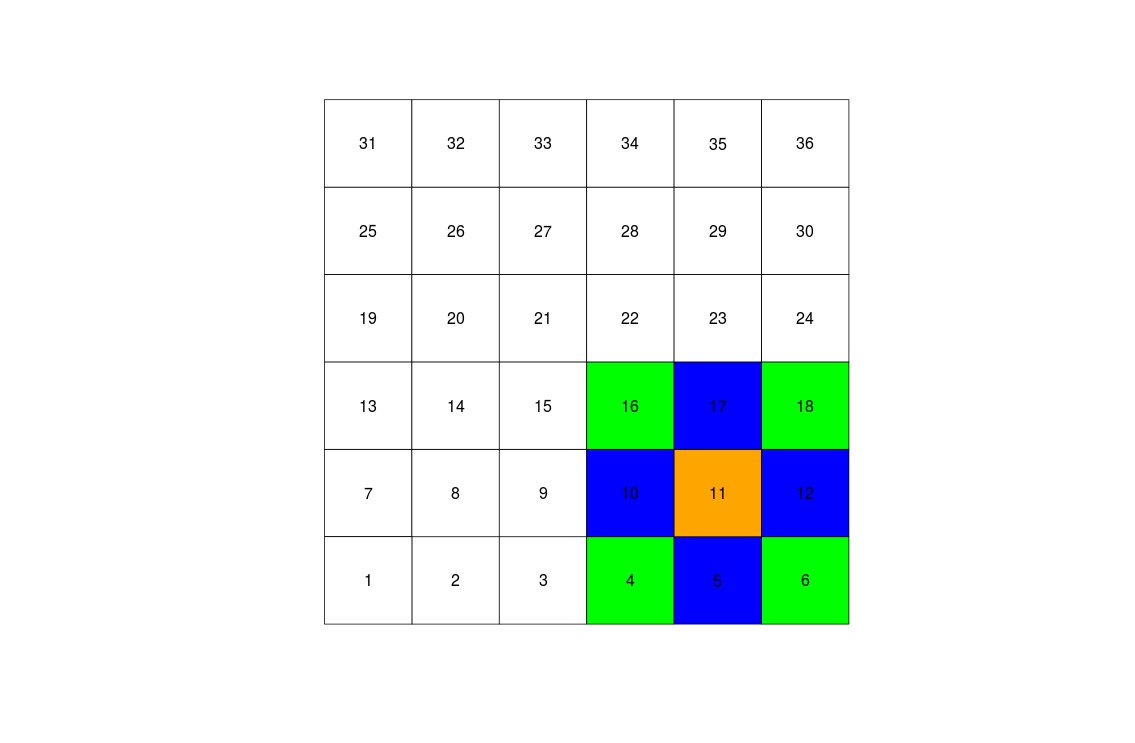
\includegraphics[scale=0.4]{Demo_Circular}\\
		\caption{Demonstration for Circular. 
			Start with the centroid at region 11, we increase the radius up to 1.5 unit. For the radius of 1, regions 10,12,5,17 are the nearest neighbors of region 11.
			Then we increased the radius up to 1.5, regions 4,6,16,18 are the nearest neighbors of region 1.
		 \label{f:gull}}
		
	\end{figure}
	
	In this example,three candidate zones that are formed: \\
	\begin{enumerate}

	
	\item Candidate zone 1: region 11\\
	\item Candidate zone 2: Regions 11,5,10,12,17\\
	\item Candidate zone 3: Regions 11,5,10,12,17,4,6,16,18\\
	
	\end{enumerate}
	 
	 \item  \textbf {Upper Level Set (ULS) Scan Statistic :} \\
			The ULS scan statistic is an adaptive approach in which the parameter space is reduced by using the empirical cell rates,
\[
			 \hat{r_i} = \dfrac{Y_i}{n_i}
\]
			They define the Upper Level Set is the set that comprises all the regions with each level $g$.\\
			\[
U_g = \{ i : \hat{r_i} > g\}
			\]
 Within each Upper Level Set, they form their target zones as the following: \\ 
				
				Let $ULS= \{1,2,\dots,t\}$ be the Upper Level Set of regions $i$ such that $\hat{r_i} \leq \hat{r_j}$ if and only if $i < j$.  
				\begin{enumerate}
					\item Region $1$ is the first zone $Z_1$. 
					\item If region $2$ connects to region $1$, then $2 \in Z_1$. If region $2$ does not connect with region $1$, then $2$ is $Z_2$. 
					\item Keep repeating this process until we run out of regions in the ULS. \\   
				\end{enumerate}
			 In this method, the searching is reduced down to only $t$ number of regions, where $t$ is the the cardinality of a ULS set, instead of $N$.The total number of possible zones is less than or equal $t$, which is feasible to conduct a search. And a zone is a cluster within $U_g$ if it has the highest T-value and is statistically significant compared to other zones within set $U_g$.\\ 
		An advantage of this method is the running times while searching can be much smaller. There are maximum $t(k)$ times and $t \leq N$. Note that $k$ is the maximum number of regions included in a zone. \\	
		However, there is a disadvantage in that we do not consider all regions as starting places.\\
		
		If we look at this method from graph theory point of view, a ULS set is a simple planar graph $H$. And our potential zones are the components $\{C_i\}_{i=1}^{t}$ of $H$. Also, each component $C_i$ has the same properties as each induced connected subgraph $G[H]$ in the circular scanning test. \\  
				
	
	The figure below is a demonstration of the scanning process of the ULS method. We set $g = \dfrac{Y_+}{n_+}$ .\\
	\begin{figure}[!ht]
		
		\centering
		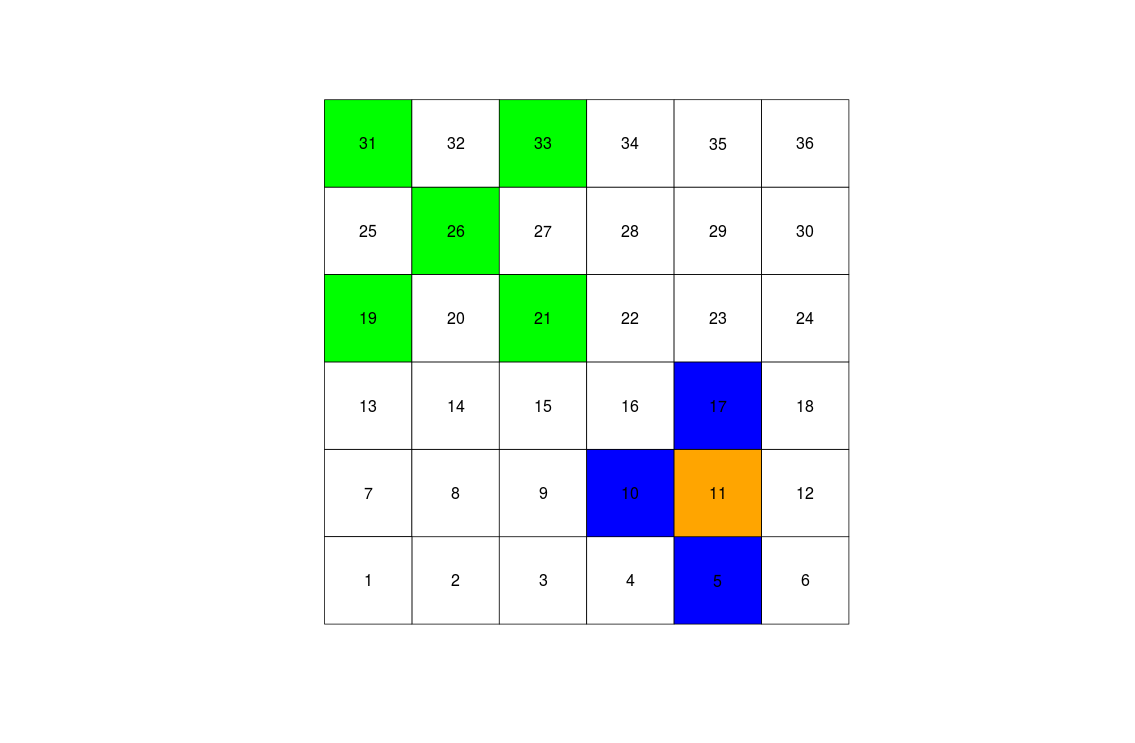
\includegraphics[scale=0.4]{Demo_ULS}\\
		\caption{Demonstration for ULS \label{f:gull}}
		
	\end{figure}
	
	
	
	Yellow regions are regions whose $G_i$ is greater than g. In this example, there are 9 regions whose $r_i >= g$ which are 17,33,21,10,5,26,31,19, and 11 in the descending order with respect to $r_i$. Firstly, region 17 is the first candidate zone. Then region 33 does not connect to 17, so region 33 creates second candidate zone. Region 21 does not connect to 17 or 33, it forms the third candidate zone. Similarly regions 10 and 5 is the 4th and 5th candidate zone respectively. Since region 26 connects to region 21 and 33, they together form a candidate zone 2*. Region 31 connects to 26, so region 31 belongs to candidate zone 2*. Region 19 also connects to region 26, which implies 19 is included in zone 2*. Finally, region 11 connects to regions 5, 10 and 17. Thus these four regions form a candidate zone 1*. Therefore, as a result we have total 7 number of candidate zones.   
		\item \textbf{ Flexible Scanning Test:}	\\
			
			The flexible scanning test is a different method to pick up potential zones for clusters. In this method,the scanning window of each region $i$ comprises a maximum $k$ regions which includes region $i$ and the $k-1$ nearest neighbors of region i. Within these $k$ regions, a cluster is the zone whose included connected regions are a subset of the $k$ regions and are connected and has the highest test statistic compare to other zones of these $k$ regions. Thus, the potential zones can have a different shape rather than a circle, which the author of this method claims better than the circular method. \\
			
				Let $Z_{ik}$ denote the zone composed region $i$ and its nearest ${k-1}$ neighbors. Windows are scanned by the spatial scan statistic are included in the set : \\
		\[
			Z = \{Z_{ik} | 1 \leq i \leq N, 1 \leq k \leq K \}
		\] 
				In this method, the maximum number of regions that are searched equals $N*$(number of connected zones that include region $i$ and the total number of regions in them are less or equal $k$) , which makes the clustering searching slower. However, this is quite a small number of zones compare to possible $2^{\binom{n}{2}}$ zones we could have in this study area. \\
			
			In graph theory's language, clusters in this method are induced connected subgraphs of $G$ which have less than or equal $k$ number of vertices, and for which extend no further than $k$ from vertex $i$.\\
			 	
	
	The figure below is a demonstration of the scanning process of the Flexible method. Again, the original region is 11, and we set the maximum number of regions for each zone is $k=6$.\\
	\begin{figure}[!ht]
		
		\centering
		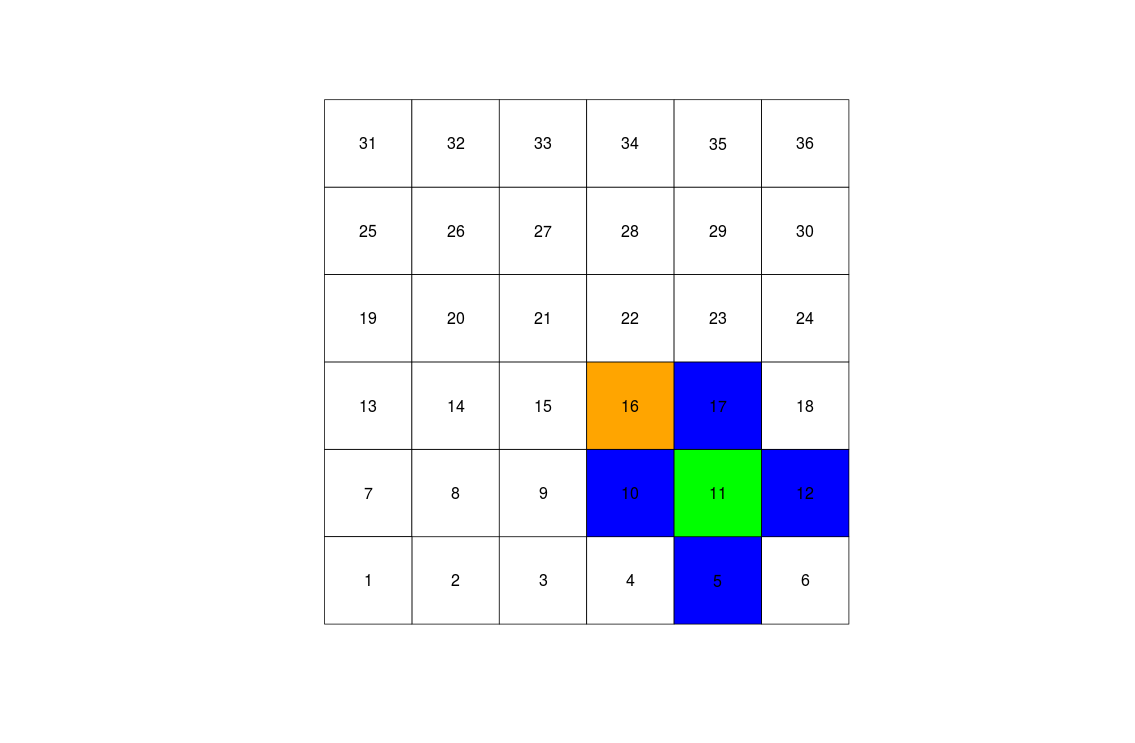
\includegraphics[scale=0.2]{Demo_Flexible}\\
		\caption{Demonstration for Flexible with k=6 \label{f:gull}}
		
	\end{figure}
	
	
	
	In this demonstration, we choose region 11 as the center region, then pick the $5$ nearest regions to 11 is 10,12,5,7 and 16. Now we will find all connected zones that include region 11 to be the candidate zones.  \\  
	
	In this example, we generated $23$ candidate zones which are: \\
	

		
	\begin{figure}[!ht]
\hspace{2cm}\begin{tabular}{|c|c|c|c|}

		\hline
		Candidate zone & Regions & Condidate zone & Region \\
		\hline
		1 & 11 & 14 & 11,5,12,17 \\
		2 & 11,5 & 	15 & 11,12,5,10 \\
		3 & 11,10 & 16 & 11,5,17,10 \\	
		4 & 11,12 & 	17 & 11,5,12,18 \\\
		5 & 11, 17 & 18 & 11,10,12,18  \\
		6 &  11,5,10 & 19 &  11,12,17,18,5  \\
		7 & 11,5,12 & 20 &   11,12,7,18,10  \\
		8 & 11,10,17 & 21 & 11,10,12,5,18 \\
		9 & 11,12,17  & 22 & 11,10,5,17,18 \\
		10 & 11,5,17 &   23& 11,5,12,10,17 \\
		11 & 11,10,12 & &\\
		12 & 11,12,17,18 & &\\
		13 & 11,12,10,17 & &\\
		
		\hline
		\end{tabular}
		
	\caption{This is the list of the 23 candidate zones generated using the above demonstration. \label{f:gull}}	
	\end{figure}

\newpage
	\section{A Contrast of the Three Methods Applied on the Leukemia New York Data}
	In this section, using the Leukemia New York data, we take a closer look at the differences among these three methods in determining their own clusters. \\
	The table below shows clusters of each method:\\
	
	\begin{tabular}{|c|c|c|c|}
	\hline
	& Circular & ULS & Flexible \\
	
	 & 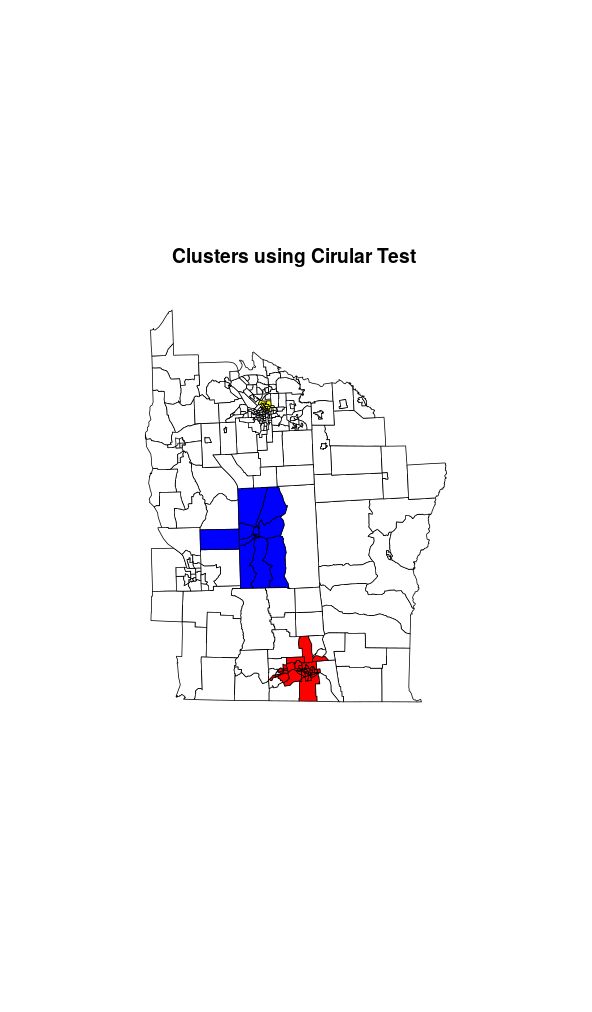
\includegraphics[scale=0.3]{cluster_circular} & 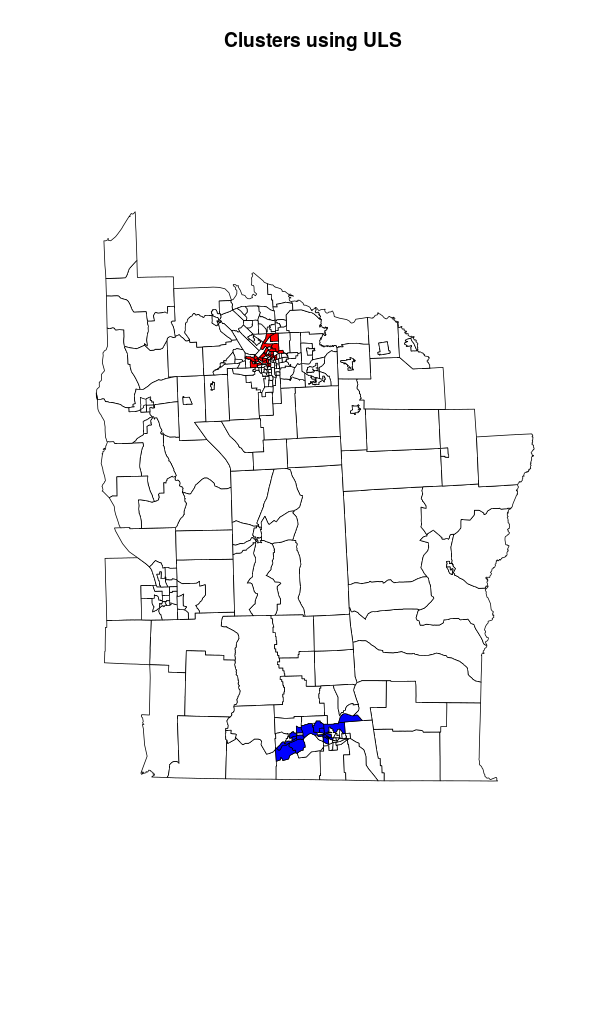
\includegraphics[scale=0.2]{cluster_uls} & 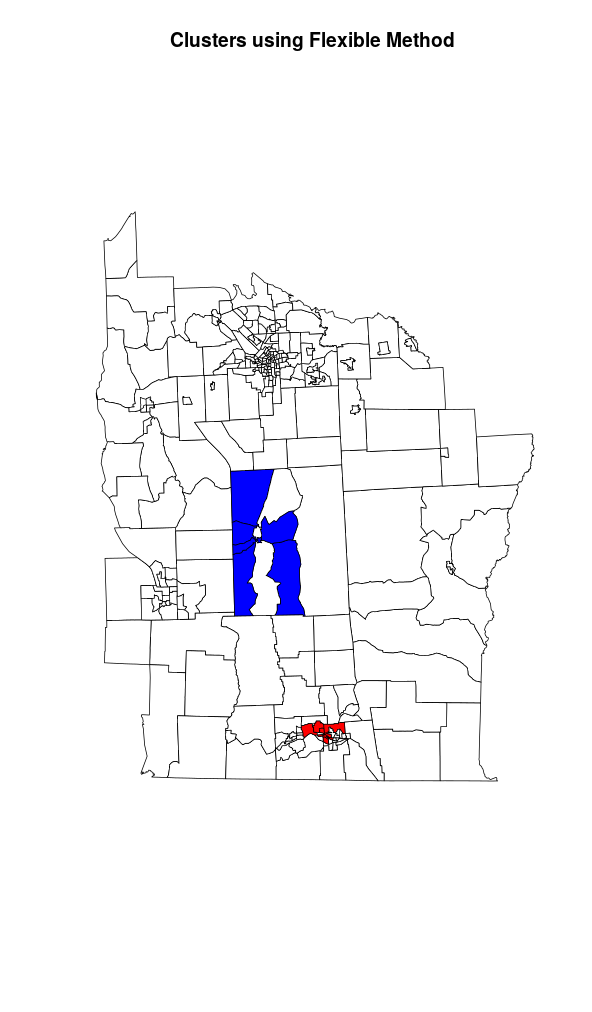
\includegraphics[scale=0.2]{cluster_flexible}\\
	\hline
	\end{tabular}
	
	 \subsection {Circular Method} 
	
	 \begin{tabular}{|c|c|c|c|c|}
	 \hline
	 & Observed Cases & Population & Log of T-value& P-value  \\
	Cluster 1: & 117 & 135295 & 15.00556 & 0.01\\ 
	Cluster 2:& 47 & 48501 & 7.851015 & 0.09\\
	Cluster 3:& 44 & 45667 & 7.199672 & 0.1\\
	\hline
	\end{tabular} \\
	
	\subsection{Upper Level Set Method} 
	
	 \begin{tabular}{|c|c|c|c|c|}
	 \hline
	 & Observed Cases & Population & T-value &P-value  \\
	Cluster 1: & 78 & 66679 & 21.61002 & 0.01\\ 
	Cluster 2:& 73 & 62749 & 19.86723 & 0.03\\
	% Cluster 3:& &  &  &\\
	\hline
	\end{tabular} \\
	
	\subsection{Flexible Method} 
	
	 \begin{tabular}{|c|c|c|c|c|}
	 \hline
	 & Observed Cases & Population & T-value & P-value  \\
	Cluster 1: & 39 & 31420 & 11.67128& 0.01\\ 
	Cluster 2:& 43 & 36446 & 11.64168 &\\
	 % Cluster 3:& &  &  &\\
	\hline
	\end{tabular} \\
	
	
	\textbf{Circular Scanning Method:} Three clusters have circle-like shapes, and each cluster includes more regions than the other two methods.\\
	\textbf{ULS Scanning Method:} The shape of the two clusters are different than circles. \\
	\textbf{Flexible Scanning Method:} The maximum number of regions for each cluster is restricted at 15.	
	The shapes of clusters in this method are more flexible than the circle shape in Circular Scan Method. These clusters overlap with clusters from the circular scanning, except it has only two instead of three clusters. \\
	
	\section{A Small Example}
	Although we have access to the Leukemia dataset, it is easier to contrast the three methods using a smaller scale dataset for which the true clusters are known. This section will help us to see in a smaller example how each method pick up the clusters. We created a dataset of a study area having 36 regions. The spatial setup of this dataset is a $6\times6$ grid. The population for each region was randomly generated using Poisson distribution with the mean of 1 million. We picked in advance 2 true clusters. One cluster had 4 connected regions and the other one had 3 connected regions. The observed cases for each region was generated as the following: \\
		
	\begin{tabular}{|c|c|}
	\hline
	Regions & Observed Cases \\
	\hline
	7,11,12,17(Cluster 1) and 20,26,32(Cluster 2) & Observed cases = 0.005 * population \\ 
	4,5,10,14,15,18,24,23 & Observed cases = 0.002 * population \\
	1,2,3,6,8,9,13,19,21,22,25,26,28,29,30,31,33,34,35,36 & Observed cases = 0.001 * population \\
	\hline
	\end{tabular}	
	
	\end{enumerate} 

		
		
	\begin{figure}[!ht]
	\centering
	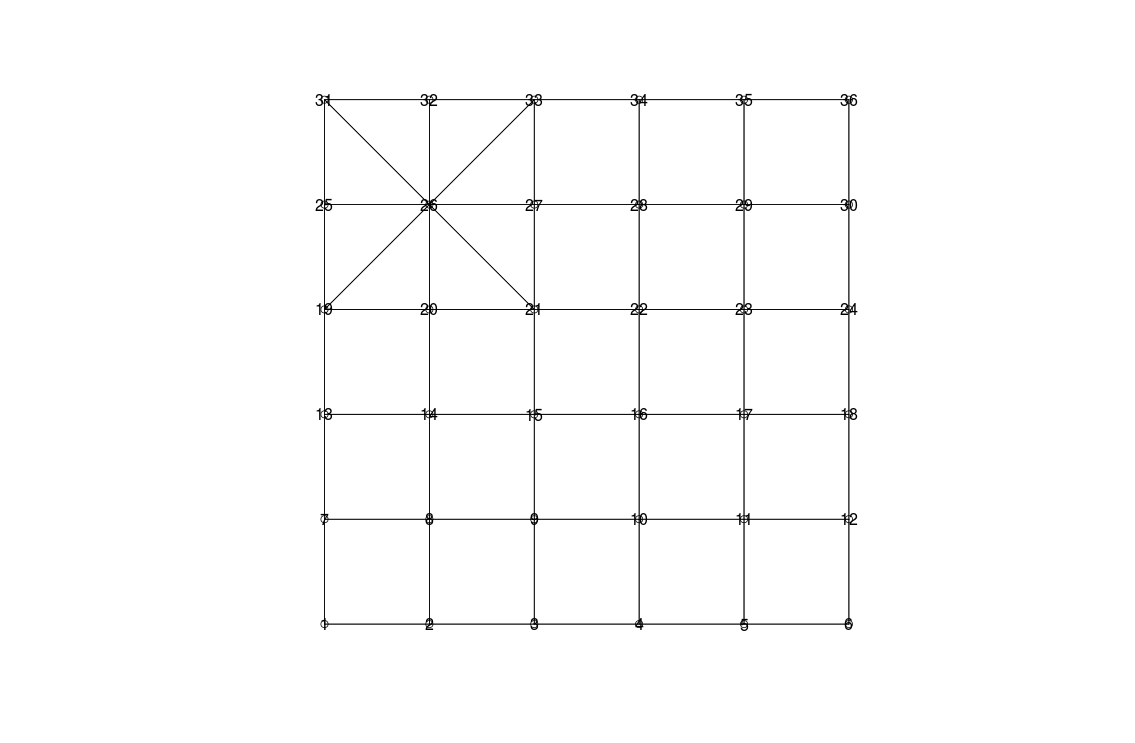
\includegraphics[scale=0.3]{Area_layout}\\
	\caption{Study Area layout. This is the layout of our study area for our small examples.\label{f:gull}}	
		\end{figure}
	
	And the figure below shows the density of the observed cases of each region in the entire study area.\\
	
	\begin{figure}[!ht]
		
		\centering
		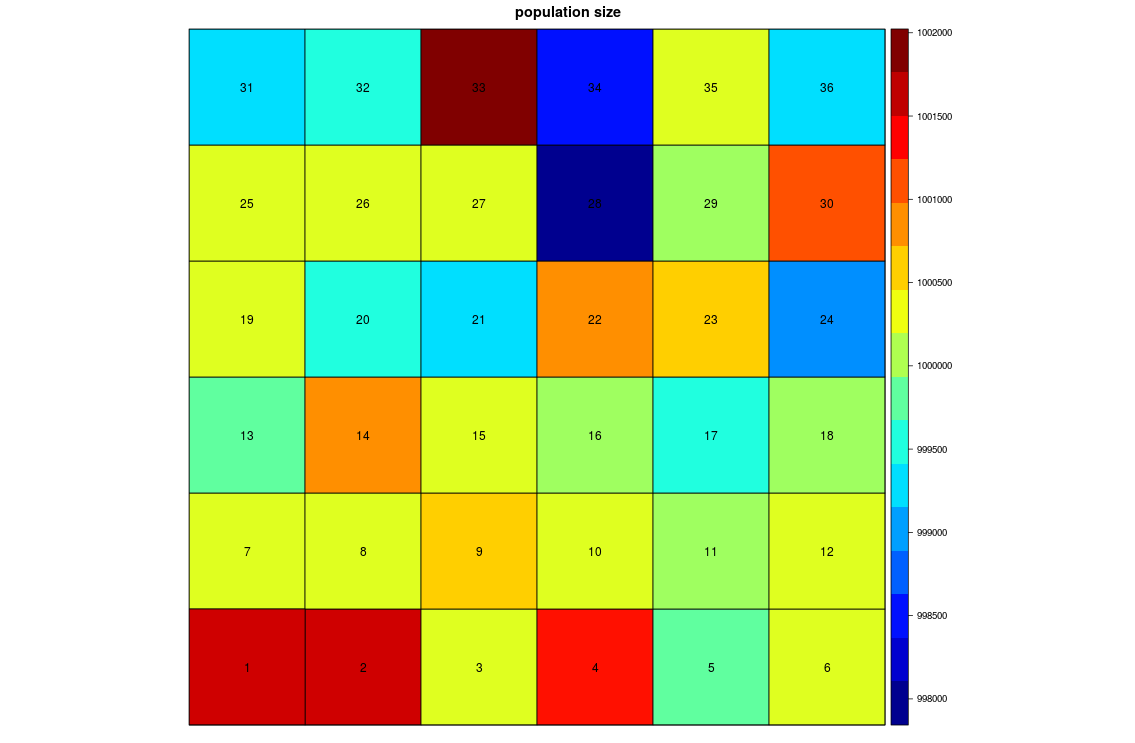
\includegraphics[scale=0.2]{Population}\\
		\caption{Population size.\label{f:gull}}
		
	\end{figure}
	
	
	As we deliberately determined the two true clusters, the closest picture of our study area should have looked like the below graph: \\
	
	\begin{figure}[!ht]
	\centering
	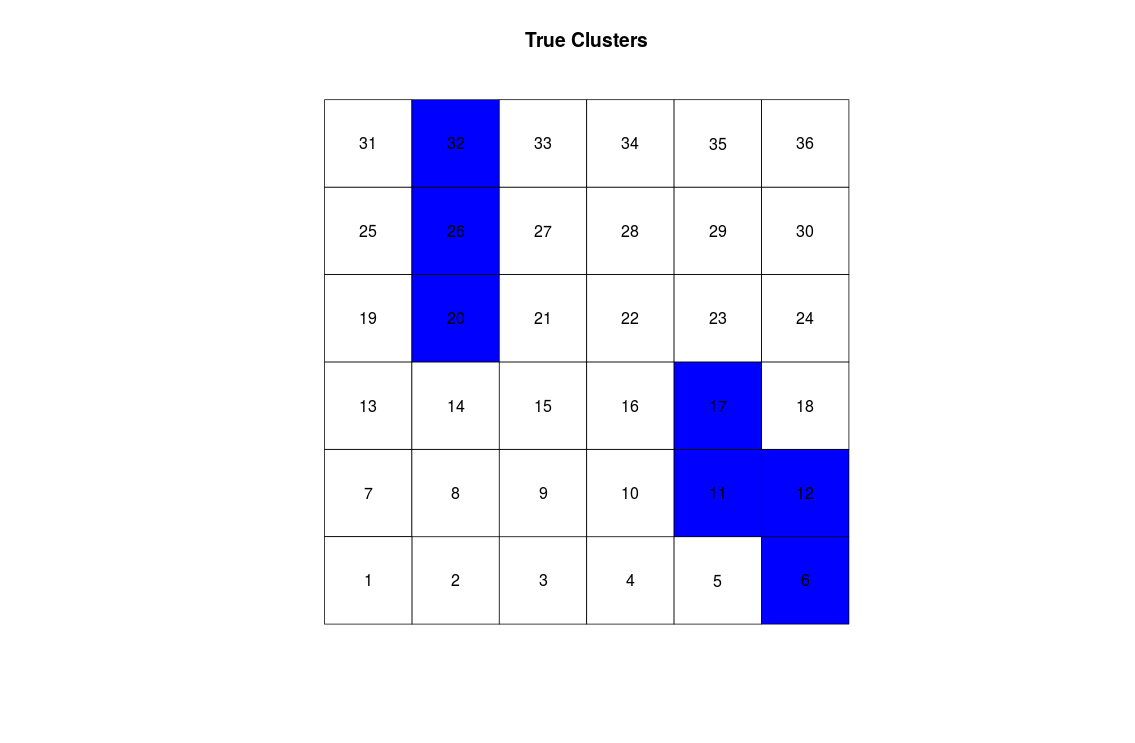
\includegraphics[scale=0.25]{Ex1_True}\\ 
	\caption {The true clusters. The connected blue nodes were divided into the two separating clusters.\label{f:gull}}
	 \end{figure}

	Then we tested the three methods using this dataset. \\
	
\subsection{Clusters of Circular Test } 
	 
	 \begin{figure}[!ht]
	 	
	 	\centering
	 	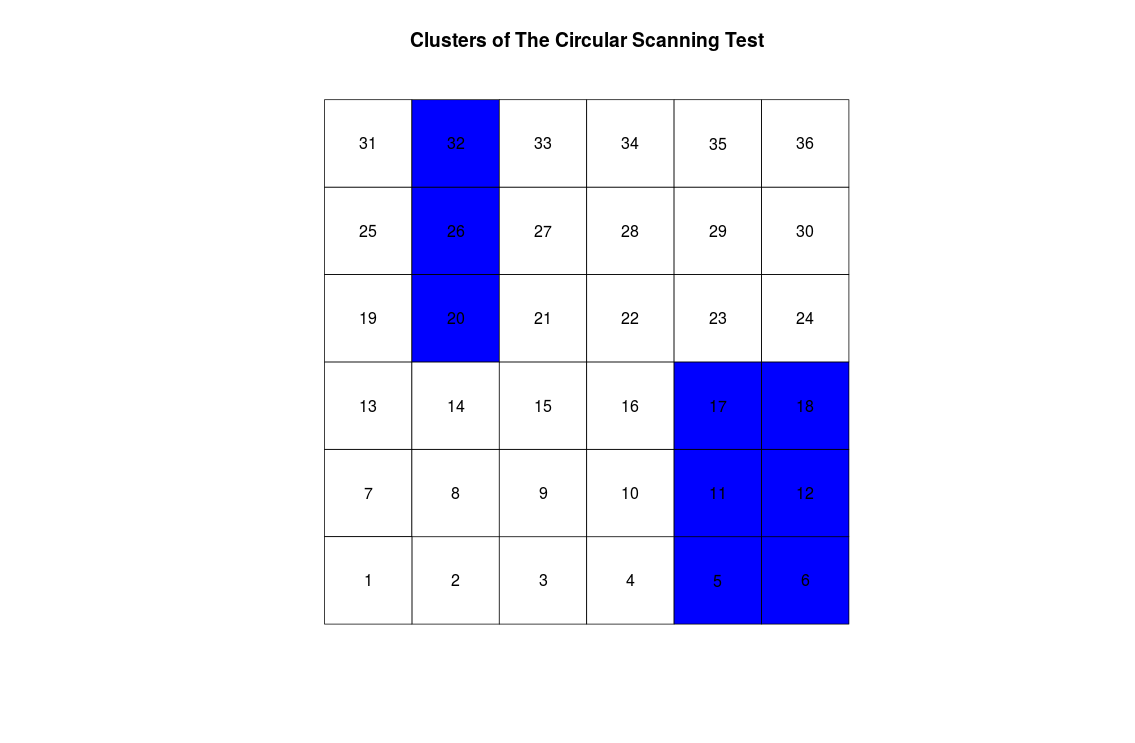
\includegraphics[scale=0.2]{Ex1_Circular}\\
	 	\caption{Clusters of Circular Scanning Test.The circular method produced two clusters. One had 6 connected regions, and the other one had 3 connected regions. This method detected one true cluster. and it also detected the second true cluster but added two extra regions to it.\label{f:gull}}
	 	
	 \end{figure}
	 
	 
\subsection{Clusters of ULS Test}
		
	
	
		\begin{figure}[!ht]
			
			\centering
			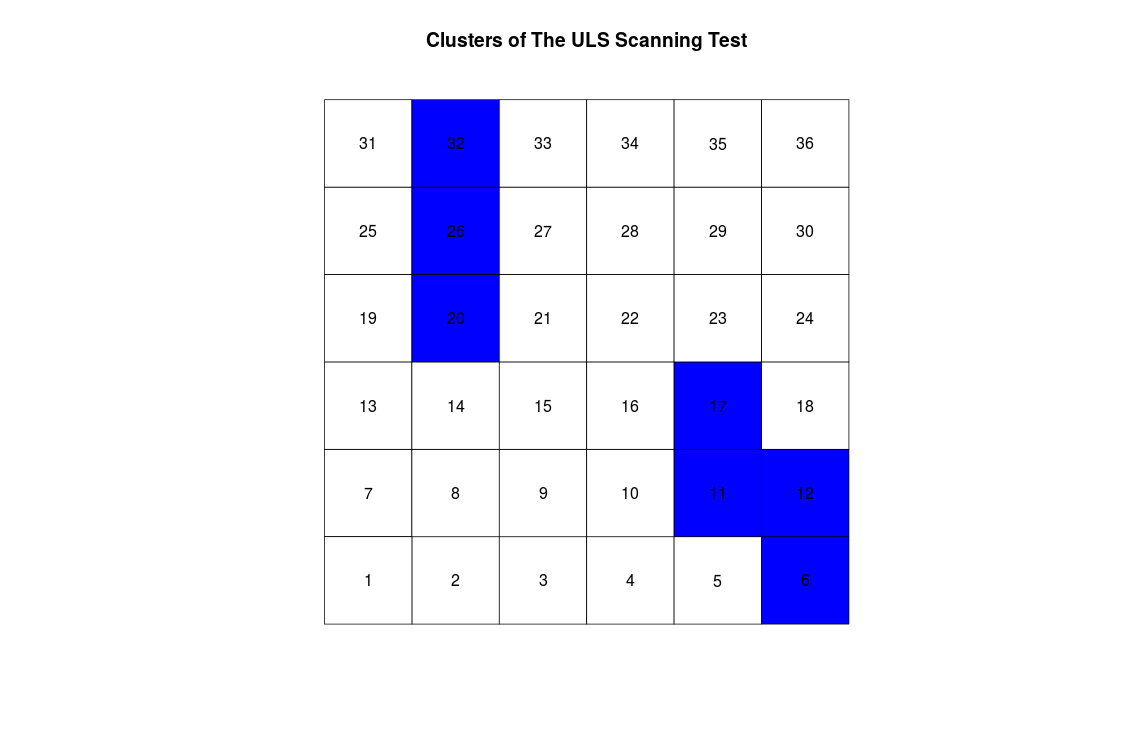
\includegraphics[scale=0.2]{Ex1_ULS}
			\caption{Clusters of the ULS Scanning Test. This method detected two clusters using a population upper bound of $10\%$ of the total population(ubpop = 0.1).This results perfectly match the true clusters. \label{f:gull}}
			
		\end{figure}	
	

		 
	 
\subsection{Flexible Scanning Test}	


\begin{figure}[!ht]
	\centering
	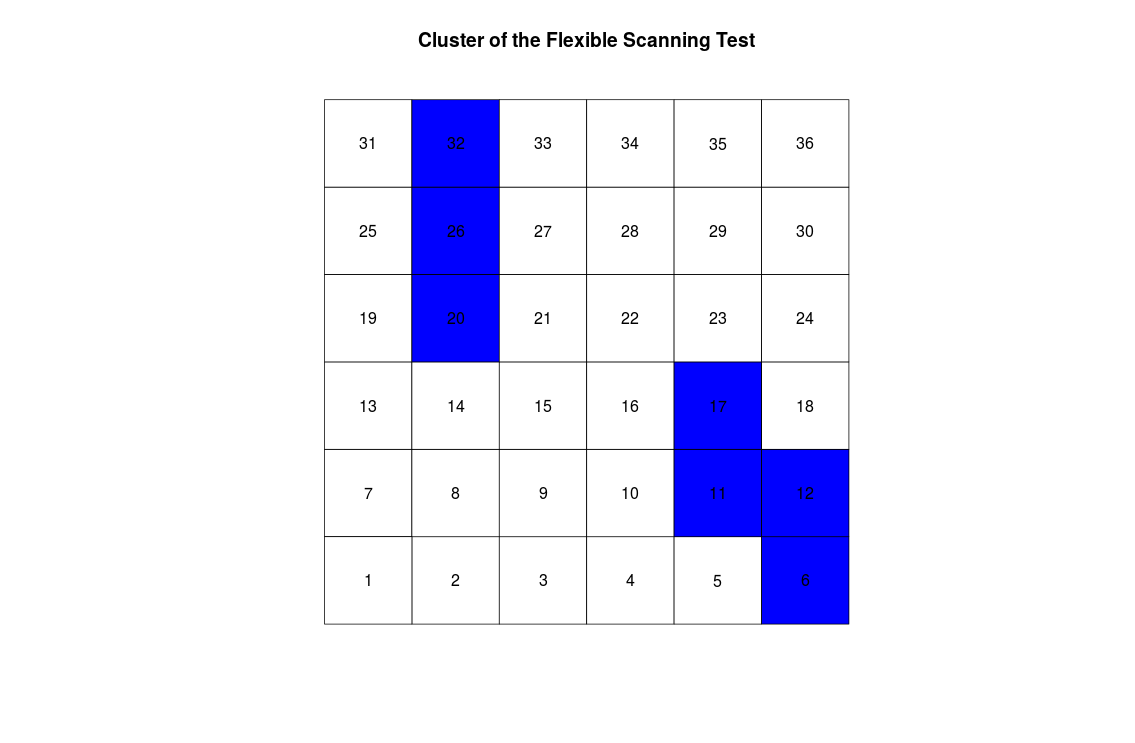
\includegraphics[scale=0.2]{Ex1_Flexible}
	\caption{Cluster of the Flexible Scanning Test.We found these two clusters when we ran this test with k=4 which were the true clusters.\label{f:gull}}
\end{figure}
	




\section{Conclusion}

In this small example,ULS and Flexible scanning tests detected the true clusters with an appropriate setup, while the Circular method detected two extra regions to be considered as hotspots. These results are compatible with the New York Leukemia data with respect to the size of clusters. In section 4, we found that the Circular scanning test detected larger clusters compared to clusters of the other two methods. Thus we might suspect that the Circular method tends to detect more false hot spots than the ULS and Flexible scanning tests. A possible explanation for this observation is that for Circular scanning test, candidate zones are circular shape. Thus, a detected hotspot could include a few false regions if they are in the same circle as the true hotspot.\\  

To strengthen our hypothesis, we tested another example with true clusters that had different shapes than our first example. We wanted to see if the results were consistent with our assumption about the Circular scanning test.\\ 
The following figure are shown the two true clusters.\\

\begin{figure}[!ht]
	\centering
	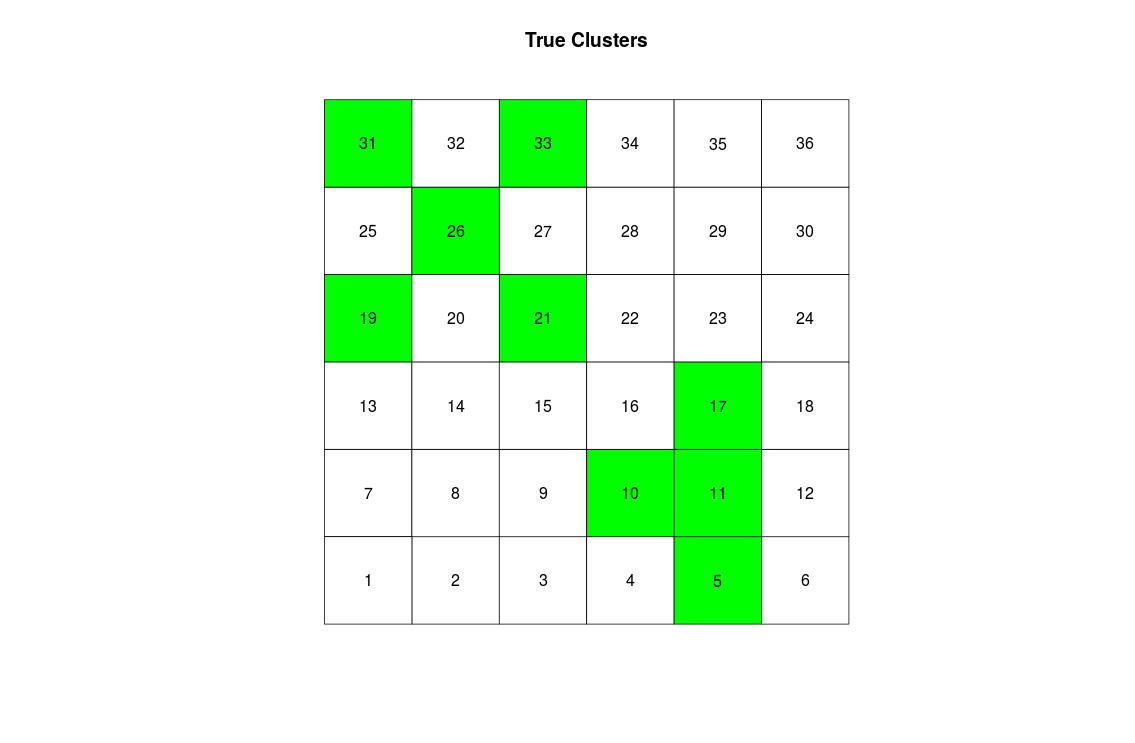
\includegraphics[scale=0.2]{Ex2_True}\\
	
	\begin{tabular}{|c|c|}
		\hline
		Cluster & Regions \\
		\hline
		1 & 19,21,26,31,33 \\
		2 & 5,10,11,17 \\ \hline
	\end{tabular} \\
	
	
	\caption{True Clusters. This is the picture of the true clusters in the second example. \label{f:gull}}
	
\end{figure}




First, we found 2 clusters using the Circular scanning test:\\


\begin{figure}[!ht]
	
	\centering
	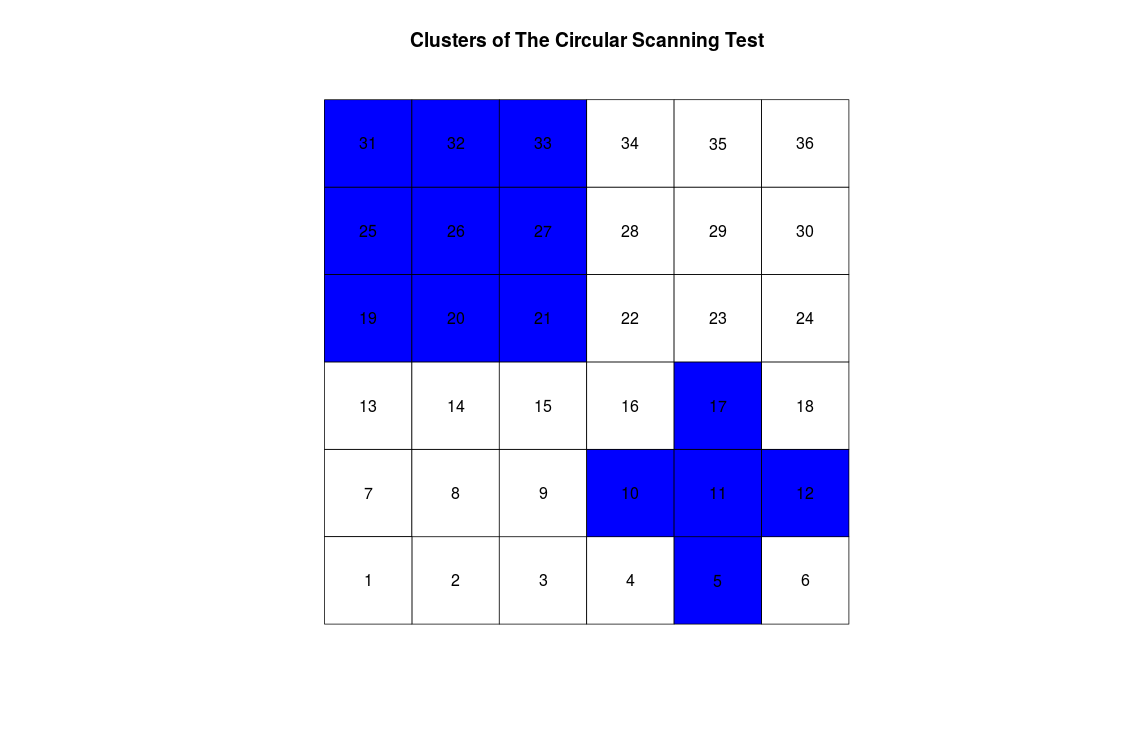
\includegraphics[scale=0.2]{Ex2_Circular}\\
	\caption{Cluster of the Circular Scanning Test.\label{f:gull}}
	
\end{figure}

\hspace{4cm}\begin{tabular}{|c|c|}
	\hline
	Cluster & Regions \\
	\hline
	1 & 19,25,20,21,26,27,31,32,33 \\
	2 & 5,10,11,12,17 \\ 
	 \hline
\end{tabular} \\

This results were not surprising us as clusters included five extra regions compared to our true clusters.\\
\newpage
The next figure illustrates the clusters of ULS method: \\ 

\begin{figure}[!ht]
	
	\centering
	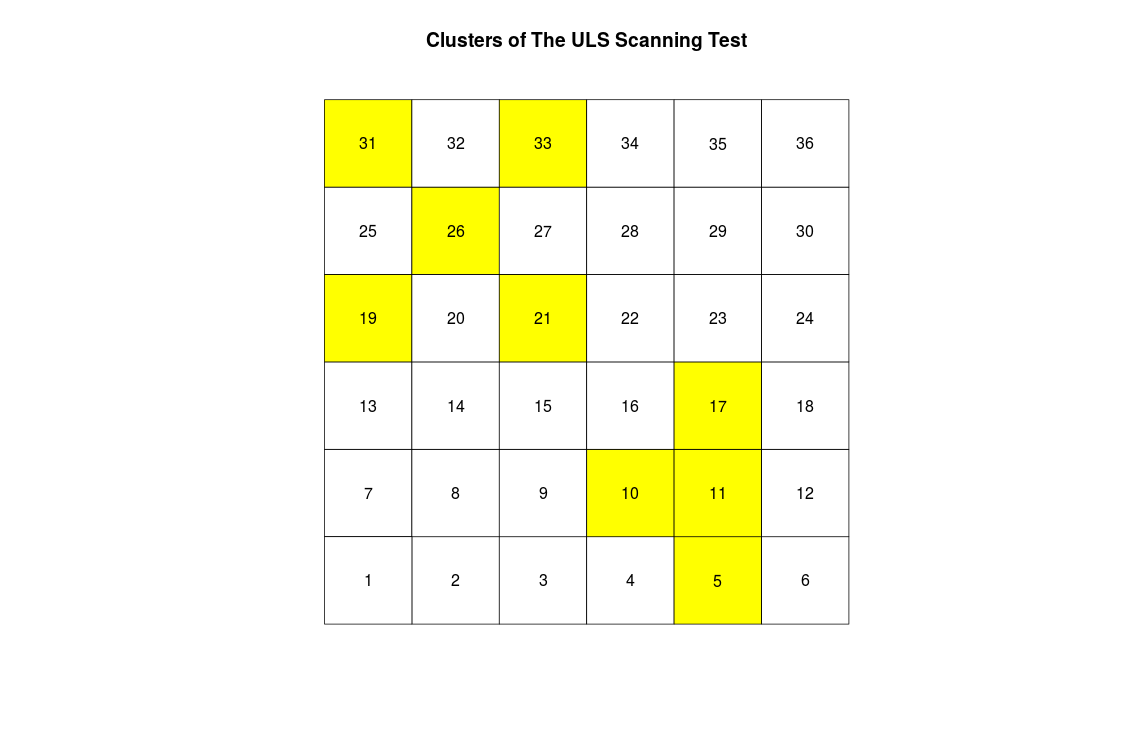
\includegraphics[scale=0.2]{Ex2_ULS}\\
	\caption{Cluster of the ULS Scanning Test. With a limit of $30 \% $  of the total population (ubop = 0.3), the ULS method picked up the true clusters.\label{f:gull}}
	
\end{figure}



\newpage


And the results using Flexible method are the following:\\

% Picture in flow 
\begin{figure}[!ht]
\centering
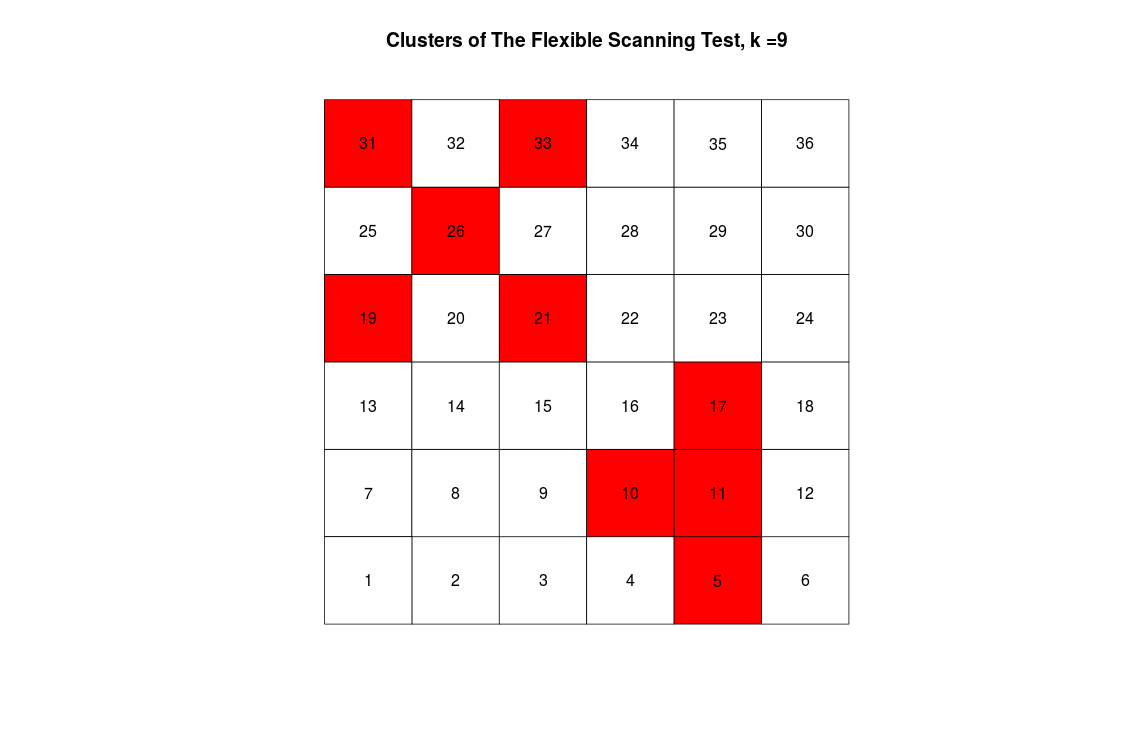
\includegraphics[scale=0.3]{Ex2_Flexible}\\
\caption{Cluster of the Flexible Scanning Test. In this example, in order for Flexible scanning test to find true clusters, we needed to increase $k$ up to 9, which was unexpected since the largest size of our true clusters was five. \label{f:gull}}

\end{figure}


So there are trade offs between using the Circular and Flexible scanning tests. The technique of selecting candidate zones of Circular method and Flexible method are similar since they tend to pick the nearest neighbors of a given center zone. However, using the Flexible scanning test, we have more candidates zones, and we can find the true clusters with less risk of including false regions. One drawback of Flexible scanning test is that it can be difficult to computationally run when the study area is big enough. On the other hand, Circular method can help us to search for clusters more quickly, even though we might include some false regions in the results. \\
   
The ULS method has the least number of candidate zones. Thus it is not quite comparable to compare and contrast to other two methods. However in our small example, this is the most effective scanning method in searching for the true clusters. \\



\section{Appendix}
\subsection{Technical Terms}
\begin{tabular}{|c|c|}
\hline
\textbf{Statistical Terminology }& \textbf{Graph Theory Terminology} \\
\hline
A Study Area & A Graph $G$ \\
A Region & A Vertex \\
A boarder & An edge \\
A Zone & An Induced Connected Sub-graph\\

\hline

\end{tabular} \\

 	
\subsection{Definitions:} 
\begin{itemize}
\item True region:  region that belongs to the true clusters. \\ 
\item False region:  region that does not belong to the true clusters. \\ 
\item Candidate zone:  one or more connected regions that is formed while a method is searching for clusters.\\ 
\item Candidate pool:  a pool that contains all the candidate zone of a method when applied to a specific study area. \\
\end{itemize}



\end{document}
